
\section{Auswertung}
\subsection{Untersuchung der Filterkurve}
Zur Bestimmung der Filterkurve des Selektivverstärkers wird die Frequenz $\su{\nu}$ gegen die Ausgangsspannung $\su{U_A}$
aufgetragen. Die Messwerte sind aus Tabelle \ref{tab:Messung1} zu entnehmen.
Aus diesen folgt die Filterkurve in Abbildung \ref{fig:filter}.
\begin{table}
  \centering
  \caption{Messwerte zur Bestimmung der Filterkurve}
  \label{tab:Messung1}
  \begin{tabular}{c c | c c}
    \toprule {$\nu\,/\,kHz$} & {$U_A$\,/\,mV} & {$\nu\,/\,kHz$} & {$U_A$\,/\,mV}\\
    \midrule
30,0 & 5,84 & 35,1 & 126,00 \\
31,0 & 6,72 & 35,2 & 138,00 \\
32,0 & 8,80 & 35,3 & 120,00 \\
33,0 & 9,12 & 35,4 & 92,00 \\
33,5 & 15,20 & 35,5 & 72,00 \\
33,8 & 18,80 & 35,6 & 58,00 \\
34,0 & 21,60 & 35,7 & 48,00 \\
34,1 & 23,20 & 35,8 & 40,00 \\
34,2 & 25,60 & 35,9 & 36,00 \\
34,3 & 28,40 & 36,0 & 32,00 \\
34,4 & 31,60 & 36,2 & 26,40 \\
34,5 & 34,30 & 36,5 & 21,60 \\
34,6 & 43,20 & 37,0 & 16,00 \\
34,7 & 50,40 & 38,0 & 9,60 \\
34,8 & 61,60 & 39,0 & 7,20 \\
34,9 & 74,00 & 40,0 & 6,00 \\
35,0 & 98,00 \\
\bottomrule
\end{tabular}
\end{table}
\begin{figure}
  \centering
  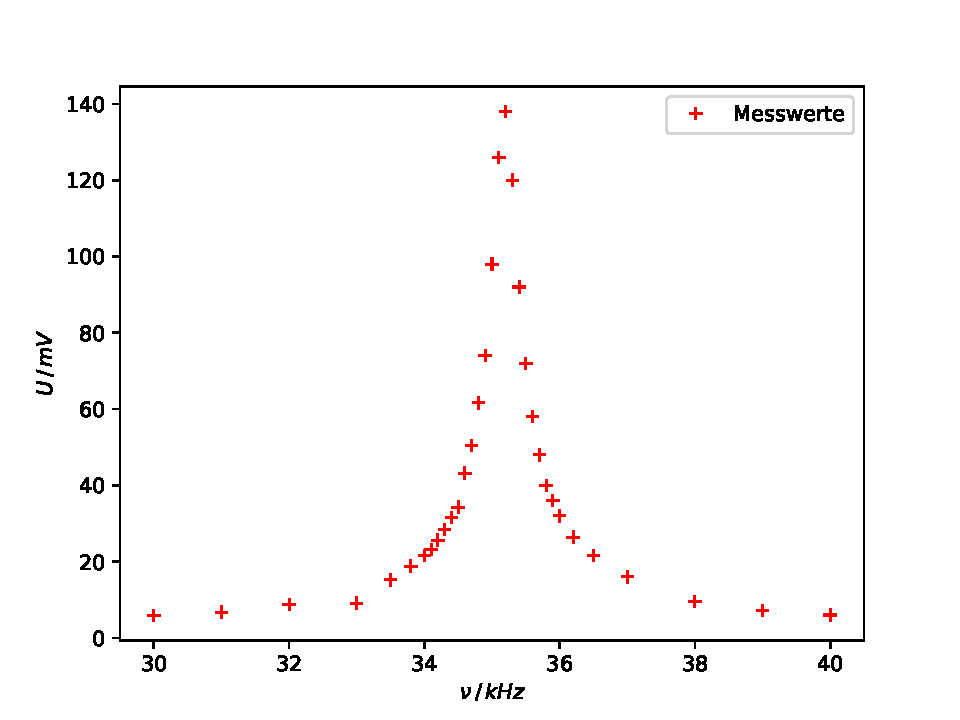
\includegraphics[scale=0.7]{filter.pdf}
  \caption{Filterkurve des Selektivverstärkers}
  \label{fig:filter}
\end{figure}
\newpage
\subsection{Experimentelle Bestimmung der Suszeptibilität}
Zur Berechnung der Querschnittsfläche werden die geometrischen Maße der Probe benötigt.
Diese sind aus Tabelle \ref{tab:geo} zu entnehmen.
\begin{table}
  \centering
  \caption{Geometrische Eigenschaften der Probe}
  \label{tab:geo}
  \begin{tabular}{c c c c}
    \toprule {$\su{Probe}$} & {$m$\,/\,g} & {$l$\,/\,cm} & {$\rho$\,/\,$\frac{g}{cm^3}$}\\
    \midrule
$\su{C_{6}O_{12}Pr_{2}}$ & 7,87 & 15,9 & 6,30  \\
\bottomrule
\end{tabular}
\end{table}
\newline
Die reale Querschnittsfläche kann dann mit Formel \ref{eqn:Q} bestimmt werden. Für diese
ergibt sich dann ein Wert von
\begin{align*}
  Q_{\su{real}} &= 78,57\,mm^2.
\end{align*}
Die aufgenommenen Messwerte für die Probe sind in Tabelle \ref{tab:Messung2} zu sehen.
\begin{table}
  \centering
  \caption{Messwerte zur Bestimmug des Suszeptibilität für $\su{C_{6}O_{12}Pr_{2}}$}
  \label{tab:Messung2}
  \begin{tabular}{c c c c c c c}
    \toprule {$\su{Messung}$} & {$U_\su{vor}$\,/\,mV} & {$U_\su{nach}$\,/\,mV} & {$\Delta{U}$\,/\,mV} & {$R_\su{vor}$\,/\,$\Omega$ } & {$R_\su{nach}$\,/\,$\Omega$} & {$\Delta{R}$\,/\,$\Omega$}\\
    \midrule
1 & 17,6 & 18,4 & 0,8 & 1,535 & 0,55 & -0,985 \\
2 & 17,6 & 16,8 & -1,2 & 1,155 & 0,24 & -0,915\\
3 & 17,6 & 17,6 & 0,0 & 0,35 & 0,16 & 0,19\\
\bottomrule
\end{tabular}
\end{table}
\newpage
Die Suszeptibilitätsbestimmung über die Spannung wird mithilfe von Formel \ref{eqn:xs}
durchgeführt.
\newline
Für die Suszeptibilät über den Widerstand wird Fomel \ref{eqn:xw} verwendet. Dabei ist der Widerstand
$\su{R_3}$ = 998\,$\su{\Omega}$.
\newline
Beide Mesungen werden drei Mal durchgeführt.
Der Mittelwert und die Standardabweichung errechnen sich dabei durch
\begin{equation}
  \bar{x} = \frac{1}{n} \sum{x_n}
  \label{eqn:Mittelwert}
\end{equation}
und
\begin{equation}
\upsigma = \frac{1}{\sqrt{n}} \sqrt{\frac{\sum{(x_n - \bar{x})^2}}{n-1} }.
\label{eqn:Standardabweichung}
\end{equation}
Für die experimentell bestimmten Suszeptibilitäten über die beiden Verfahren folgt dann
\begin{align*}
  \chi_{\su{U}} &= (9,09\pm0,30) \cdot 10^{-4} \\
  \chi_{\su{R}} &= (1,55\pm1,14) \cdot 10^{-3}.
\end{align*}
\subsection{Theoretische Bestimmung der Suszeptibilität}
Zur Berechnung des theoretischen Wertes wird zu erst der Landé-Faktor mit \ref{eqn:gj} berechnet.
Die dafür benötigten Quantenzahlen werden durch die Hund'schen Regeln festgelegt.
Um den Gesamtspin S zu berechnen, wird die Elektronenkonfiguration der nicht
abgeschlossenen Hüllen betrachtet. Dabei wird jedem Elektron einen Spin $s = \frac{1}{2}$
zugeordnet. In diesem Fall ist $S = 3 \cdot \frac{1}{2} = 1,5$.
\newline
Unter Berücksichtigung des Gesamtspins und des Pauli-Prinzips wird der Bahndrehimpuls
berechnet. Der maximale Bahndrehimpuls von 4f-Elektronen beträgt $l_{\su{max}} = 3$.
Da $\su{C_{6}O_{12}Pr_{2}}$ drei freie 4f-Elektronen besitzt, folgt für den Gesamtbahndrehimpuls
\newline
$L = 3+2+1 = 6$.
\newline
Da die Schale weniger als die Hälfte gefüllt ist, wird der Gesamtdrehimpuls durch
\newline
$J = L-S = 6-1,5 = 4,5$ bestimmt.

Nach der Bestimmung des Landé-Faktors kann mit Formel \ref{eqn:xw} die theoretische Suszeptibilität
berechnet werden. Dafür wird der Zusammenhang für die benötigte Anzahl pro Volumeneinheit N
benötigt. Es ergibt sich
\begin{align}
  N &= \frac{\rho}{M}.
\end{align}
M ist hierbei die molare Masse der Probe und beträgt 545,8723u \cite{Wert}.
\newline
In der folgenden Tabelle \ref{tab:qua} sind die Quantenzahlen, sowie die benötigte Anzahl
pro Volumeneinheit und der Landé-Faktor aufgelistet.
\begin{table}
  \centering
  \caption{Quantenzahlen und Landé-Faktor}
  \label{tab:qua}
  \begin{tabular}{c c c c c c c}
    \toprule {Probe} & {M /$10^{-25}$kg} & {N /$10^{27}$ 1/$m^{3}$}  & {L} & {S} & {J} & {$g_j$}\\
    \midrule
$\su{C_6 O_{12} Pr_{2}}$ & 9,064 & 6,95 & 6 & 1,5 & 4,5 & 0,73 \\
\bottomrule
\end{tabular}
\end{table}
Danach wird unter der Annahme $T= 293.15\,K$ die theoretisch Suszeptibilität von $\su{C_{6}O_{12}Pr_{2}}$
bestimmt. Es folgt
\begin{align*}
  \chi_{\su{theoretisch}} &= 8,09 \cdot 10^{-4}.
\end{align*}
\section{Diskussion}
In der folgenden Tabelle \ref{tab:suszis} sind die bestimmten Suszibilitäten und die jeweilige
Abweichung zum Theoriewert dargestellt.
\begin{table}
  \centering
  \caption{Vergleich der bestimmten Suszeptibilitäten für $\su{C_{6}O_{12}Pr_{2}}$}
  \label{tab:suszis}
  \begin{tabular}{c c c c}
    \toprule {} & {$\chi_{\su{experimentell}}$} & {$\chi_{\su{theoretisch}}$} & {Abweichung / \%}\\
    \midrule
    $\chi_{\su{U}}$ & $(9,09\pm0,30) 10^{-4}$ & $8,09\cdot10^{-4}$ & 12,36 \% \\
    $\chi_{\su{R}}$ & $(1,55\pm1,14) 10^{-3}$ & $8,09\cdot10^{-4}$ & 91,59 \% \\
\bottomrule
\end{tabular}
\end{table}
\newline
Für die über die Spannung bestimmte Suszeptibilität kommt es zu einer recht geringen Abweichung vom
Theoriewert. Hier beträgt die prozentuale Abweichung ungefär 12\%. Dies lässt sich durch den
gemessenen Spannungsunterschied erklären. Zwischen dem Abgleichen der Brücke und dem Hinzufügen
der Probe hat sich die Spannung kaum bzw gar nicht verändert.

Für die über den Widerstand berechnete Suszeptibilität liegt die prozentuale Abweichung bei 92\%.
Diese große Abweichung lässt sich vor Allem durch die ungenaue Justierung des regelbaren Widerstands erklären.
Der Widerstandsunterschied zwischen abgeglichener Brücke und dem Abgleichelement war bei jeder Messung sehr groß.
Besonders bei den ersten beiden Messung ist dies der Fall. Allerdings sind diese in derselben Größenordnung.
Nur bei der dritten Messung war diese Differenz geringer und weicht dadurch deutlich von den vorherigen Messungen ab.
Ein Grund dafür ist vermutlich die gleichbleibende Spannung.

Die Filterkurve des Selektivverstärker entspricht dem erwarteten Verlauf. Deutlich ist der klare Peak und die
flachen Ausläufe zu erkennen.
